\section{Tracking Techniques}
\label{sec:tracking-techniques}

\begin{table*}[ht]
  \small
\centering
\caption{Web tracking artifact taxonomy: mapping of tracked artifacts to artifact labels.}
\label{tab:artifact-taxonomy}
\renewcommand{\arraystretch}{1.2}
\begin{tabular}{@{} p{3.4cm} p{13.8cm} @{}}
\toprule
\textbf{Artifact Label} & \textbf{Artifacts Observed in the Literature Review} \\
\midrule

Browser Storage \& Cache &
  \textit{Cookies};
  \textit{Web Storage} (localStorage, sessionStorage, IndexedDB);
  \textit{Browser Caches} (HTTP, HSTS, favicon, Alt-Svc, Service Worker, and Cache API) \\

\midrule

JavaScript-Accessible Browser APIs &
  \textit{Fingerprinting APIs} (e.g., Navigator, Screen, Canvas, WebGL, AudioContext);
  \textit{Device APIs} (Battery Status, Media Devices, Gamepad, Speech Synthesis voices); 
  \textit{Browser Permissions} (e.g., camera, microphone) \\

\midrule

Hardware Artifacts &
  \textit{GPU Rendering Behavior} (timing variations, memory allocation, performance counters);
  \textit{Sensor Calibration Data} (accelerometer or gyroscope imperfections, speaker frequency response);
  \textit{Clock Drift Patterns} (system time offset, TCP timestamp skew);
  \textit{CPU Microarchitectural State} (scheduling statistics, memory footprint) \\

\midrule

Network Protocol Artifacts &
  \textit{IP Address};
  \textit{TLS/SSL Handshake Parameters} (cipher suites, SNI, client certificates);
  \textit{TCP/IP Stack Characteristics} (source port selection, IP ID fields, IPv6 flow labels);
  \textit{DNS Records} (CNAME records, reverse hostnames, TTL values);
  \textit{QUIC/HTTP2+ Transport Metadata} (connection IDs, retry tokens, transport parameters) \\

\midrule

HTTP Traffic Artifacts &
  Request Metadata, Response Content, Headers, Payload \\

\midrule

Navigational Artifacts &
  \textit{URL Components} (host, domain, path, query parameters);
  \textit{Redirect Chains} \\

\midrule

Webpage Artifacts &
  \textit{Resources} (DOM elements and their modifications, stylesheets, scripts);
  \textit{Interaction Patterns} (click traces, touch gesture characteristics, keystrokes, mouse movements, scroll depth, click coordinates, interaction timing);
  \textit{Rendering Characteristics} (font rendering, CSS feature detection, element bounding dimensions) \\

\midrule

Identifiers &
  \textit{Authentication IDs} (OAuth tokens, SSO redirect parameters, session IDs);
  \textit{PII} (email addresses, phone, PII hashes);
  \textit{Device-specific IDs} (IDFA, EMEI, MAC address); 
  \textit{Advertiser-specific IDs} (e.g., UUIDs)\\

\bottomrule
\end{tabular}
% \vspace{-2mm}
\end{table*}


%%
Our approach described in \autoref{sec:methodology} to systematize 58 papers on specific web tracking techniques, complemented by 108 measurement studies that characterize their real-world aspects, yields 24 distinct tracking techniques, mapped in~\autoref{tab:technique-papers}.
%
Fundamentally, each tracking technique relies on artifacts tied either to the user, their device, or their browsing activity.
%
To this end, we systematize the artifacts that trackers are observed to rely on across different papers into eight categories (\autoref{tab:artifact-taxonomy}).
%
\autoref{tab:artifact-capability-matrix} systematizes research to map tracker capabilities exercised over artifact categories for each tracking technique, with a paper-level breakdown represented in~\autoref{tab:paper-artifacts}. 
%
This section systematizes tracking techniques by state maintained by the trackers across different contexts.

%%
Overall, we can observe trackers to exercise \symSharing~Sharing and \symInclusion~Inclusion capabilities with nearly every technique, since a tracker must always be included directly or indirectly within a webpage and eventually exfiltrate what it collects to be able to track. 
%
On the other hand, \symStorage~Storage is essentially exclusive to the techniques we classify as stateful that require it to maintain state across contexts, while \symObservation~Observation is concentrated with the passive or out-of-band techniques (e.g., network- and hardware-oriented techniques).


%%
\begin{table*}[t]
\centering
\scriptsize
\setlength{\tabcolsep}{1pt}
\renewcommand{\arraystretch}{1}
\caption{Tracker capabilities most commonly exercised over each artifact (rows) for each tracking technique (columns). \protect\symInclusion~Inclusion, \protect\symExecution~Execution, \protect\symStorage~Storage, \protect\symSharing~Sharing, \protect\symObservation~Observation.}
\label{tab:artifact-capability-matrix}
\begin{tabular}{%
|>{\raggedright\arraybackslash}m{3.0cm}|>{\centering\arraybackslash}m{0.63cm}|>{\centering\arraybackslash}m{0.63cm}|>{\centering\arraybackslash}m{0.63cm}|>{\centering\arraybackslash}m{0.63cm}|>{\centering\arraybackslash}m{0.63cm}|>{\centering\arraybackslash}m{0.63cm}|>{\centering\arraybackslash}m{0.63cm}|>{\centering\arraybackslash}m{0.63cm}|>{\centering\arraybackslash}m{0.63cm}|>{\centering\arraybackslash}m{0.63cm}|>{\centering\arraybackslash}m{0.63cm}|>{\centering\arraybackslash}m{0.63cm}|>{\centering\arraybackslash}m{0.63cm}|>{\centering\arraybackslash}m{0.63cm}|>{\centering\arraybackslash}m{0.63cm}|>{\centering\arraybackslash}m{0.63cm}|>{\centering\arraybackslash}m{0.63cm}|>{\centering\arraybackslash}m{0.63cm}|>{\centering\arraybackslash}m{0.63cm}|>{\centering\arraybackslash}m{0.63cm}|%
}
\toprule
\multicolumn{1}{|>{\centering\arraybackslash}b{3.0cm}|}{\shortstack[c]{\textbf{Tracked}\\\textbf{Artifacts}}} & \multicolumn{1}{>{\centering\arraybackslash}b{0.63cm}|}{\rot{Third-party Cookie Tracking}} & \multicolumn{1}{>{\centering\arraybackslash}b{0.63cm}|}{\rot{Cookie Respawning}} & \multicolumn{1}{>{\centering\arraybackslash}b{0.63cm}|}{\rot{Cookie Syncing}} & \multicolumn{1}{>{\centering\arraybackslash}b{0.63cm}|}{\rot{First-party Cookie Tracking}} & \multicolumn{1}{>{\centering\arraybackslash}b{0.63cm}|}{\rot{Tracking Pixels/Tags}} & \multicolumn{1}{>{\centering\arraybackslash}b{0.63cm}|}{\rot{CNAME Tracking}} & \multicolumn{1}{>{\centering\arraybackslash}b{0.63cm}|}{\rot{Link Decorations}} & \multicolumn{1}{>{\centering\arraybackslash}b{0.63cm}|}{\rot{Bounce Tracking}} & \multicolumn{1}{>{\centering\arraybackslash}b{0.63cm}|}{\rot{Authentication-based Tracking}} & \multicolumn{1}{>{\centering\arraybackslash}b{0.63cm}|}{\rot{Cross-context Tracking}} & \multicolumn{1}{>{\centering\arraybackslash}b{0.63cm}|}{\rot{Javascript-based Tracking}} & \multicolumn{1}{>{\centering\arraybackslash}b{0.63cm}|}{\rot{Browser Fingerprinting}} & \multicolumn{1}{>{\centering\arraybackslash}b{0.63cm}|}{\rot{Extension Fingerprinting}} & \multicolumn{1}{>{\centering\arraybackslash}b{0.63cm}|}{\rot{Device Fingerprinting}} & \multicolumn{1}{>{\centering\arraybackslash}b{0.63cm}|}{\rot{Passive Fingerprinting}} & \multicolumn{1}{>{\centering\arraybackslash}b{0.63cm}|}{\rot{Kernel-based Side-channels}} & \multicolumn{1}{>{\centering\arraybackslash}b{0.63cm}|}{\rot{Network-based Side-channels}} & \multicolumn{1}{>{\centering\arraybackslash}b{0.63cm}|}{\rot{Timing-based Side-channels}} & \multicolumn{1}{>{\centering\arraybackslash}b{0.63cm}|}{\rot{Storage-based Side-channels}} & \multicolumn{1}{>{\centering\arraybackslash}b{0.63cm}|}{\rot{Behavioral Tracking}} \\
\midrule
\rh Browser Storage and Cache & \cellsym{\symStorage} & \cellsym{\symStorage} & \cellsym{\symStorage} & \cellsym{\symStorage} & \cellsym{\symStorage} & \cellsym{\symStorage} & \cellsym{\symStorage} & \cellsym{\symStorage} & \cellsym{\symStorage} & \cellsym{\symStorage} & \cellsym{\symStorage} & \ec & \ec & \ec & \ec & \ec & \ec & \ec & \cellsym{\symStorage} & \ec \\
\hline
\rh JS-Accessible Browser APIs & \cellsym{\symExecution} & \cellsym{\symExecution} & \cellsym{\symExecution} & \cellsym{\symExecution} & \cellsym{\symExecution} & \ec & \ec & \cellsym{\symExecution} & \ec & \cellsym{\symExecution} & \cellsym{\symExecution} & \cellsym{\symExecution} & \cellsym{\symExecution} & \cellsym{\symExecution} & \ec & \cellsym{\symExecution} & \ec & \cellsym{\symExecution} & \cellsym{\symExecution} & \cellsym{\symExecution} \\
\hline
\rh Webpage Artifacts & \cellsym{\symInclusion} & \cellsym{\symInclusion} & \cellsym{\symInclusion} & \cellsym{\symInclusion} & \cellsym{\symInclusion\,\symExecution} & \cellsym{\symInclusion} & \cellsym{\symInclusion} & \cellsym{\symInclusion} & \cellsym{\symInclusion} & \cellsym{\symInclusion} & \cellsym{\symInclusion\,\symExecution} & \cellsym{\symInclusion\,\symExecution} & \cellsym{\symInclusion\,\symExecution} & \cellsym{\symInclusion\,\symExecution} & \cellsym{\symInclusion} & \cellsym{\symInclusion} & \ec & \cellsym{\symInclusion} & \cellsym{\symInclusion} & \cellsym{\symInclusion\,\symExecution} \\
\hline
\rh Hardware Artifacts & \ec & \ec & \ec & \ec & \ec & \ec & \ec & \ec & \ec & \cellsym{\symExecution\,\symObservation} & \ec & \ec & \ec & \cellsym{\symExecution\,\symObservation} & \ec & \cellsym{\symExecution\,\symObservation} & \ec & \cellsym{\symExecution\,\symObservation} & \ec & \ec \\
\hline
\rh Network Protocol Artifacts & \ec & \ec & \ec & \ec & \ec & \cellsym{\symSharing} & \ec & \ec & \ec & \ec & \ec & \ec & \ec & \cellsym{\symObservation} & \cellsym{\symObservation} & \cellsym{\symObservation} & \cellsym{\symObservation} & \ec & \ec & \ec \\
\hline
\rh HTTP Traffic Artifacts & \cellsym{\symSharing} & \cellsym{\symSharing} & \cellsym{\symSharing} & \cellsym{\symSharing} & \cellsym{\symSharing} & \cellsym{\symSharing} & \cellsym{\symSharing} & \cellsym{\symSharing} & \cellsym{\symSharing} & \cellsym{\symSharing} & \cellsym{\symSharing} & \cellsym{\symSharing} & \cellsym{\symSharing} & \cellsym{\symSharing} & \cellsym{\symSharing} & \cellsym{\symSharing} & \cellsym{\symObservation} & \cellsym{\symSharing} & \cellsym{\symSharing} & \cellsym{\symSharing} \\
\hline
\rh Navigational Artifacts & \ec & \ec & \cellsym{\symSharing} & \ec & \cellsym{\symSharing} & \ec & \cellsym{\symSharing} & \cellsym{\symSharing} & \cellsym{\symSharing} & \ec & \ec & \ec & \ec & \ec & \ec & \ec & \ec & \ec & \ec & \ec \\
\hline
\rh Identifiers & \cellsym{\symStorage\,\symSharing} & \cellsym{\symStorage\,\symSharing} & \cellsym{\symStorage\,\symSharing} & \cellsym{\symStorage\,\symSharing} & \cellsym{\symStorage\,\symSharing} & \cellsym{\symStorage\,\symSharing} & \cellsym{\symSharing} & \cellsym{\symStorage\,\symSharing} & \cellsym{\symStorage\,\symSharing} & \cellsym{\symStorage\,\symSharing} & \cellsym{\symStorage\,\symSharing} & \cellsym{\symSharing} & \cellsym{\symSharing} & \cellsym{\symSharing} & \ec & \ec & \ec & \ec & \ec & \ec \\
\bottomrule
\end{tabular}
% \vspace{-2mm}
\end{table*}


%%
We organize the remainder of this section by tracked state (\autoref{tab:systematization-criteria}), discussing the evolution of each technique under three categories: \textit{stateful} tracking (\autoref{sec:stateful-tracking}), \textit{stateless} tracking (\autoref{sec:stateless-tracking}), and \textit{mixed} tracking (\autoref{sec:mixed-techniques}).
%
Within each, we highlight research gaps and identify open problems that will shape future research directions for each technique.
%
\autoref{fig:evolution-techniques} plots the evolutionary milestones underlying our systematization across tracking techniques.

%%
\subsection{Stateful Tracking}
\label{sec:stateful-tracking}


%%
\textit{Stateful tracking} techniques involve maintaining \textit{state} by storing a unique identifier in the user's browser and retrieving it or updating it across visits, using either dedicated browser-provided interfaces (e.g., cookies) or as side effects of other functionality (e.g., E-Tags, HSTS upgrades)~\cite{englehardtAutomatedDiscoveryPrivacy2018,ashkansoltaniFlashCookiesPrivacy2011,solomosTalesFaviconsCaches2021}.


%%
Historically, stateful tracking relied primarily on third-party storage, allowing the same identifier to be read across unrelated websites.
%
However, modern browsers now either block~\cite{TrackingPreventionWebKit2020} or partition third-party access to stateful APIs by origin~\cite{mdnThirdpartyCookiesPrivacy2024}, preventing trackers from storing and retrieving identifiers across sites.
%
As a result, tracking has increasingly shifted into the first-party context, where third-party services store site-specific identifiers and subsequently link them across websites using additional reconciliation mechanisms (e.g., logged-in account information).
%
Accordingly, this section systematizes stateful tracking techniques in both third- and first-party tracking contexts.












%%
\subsubsection{Cookie-based Tracking}
\label{sec:stateful-techniques-cookies}

\begin{figure}[htbp]
    \centering
    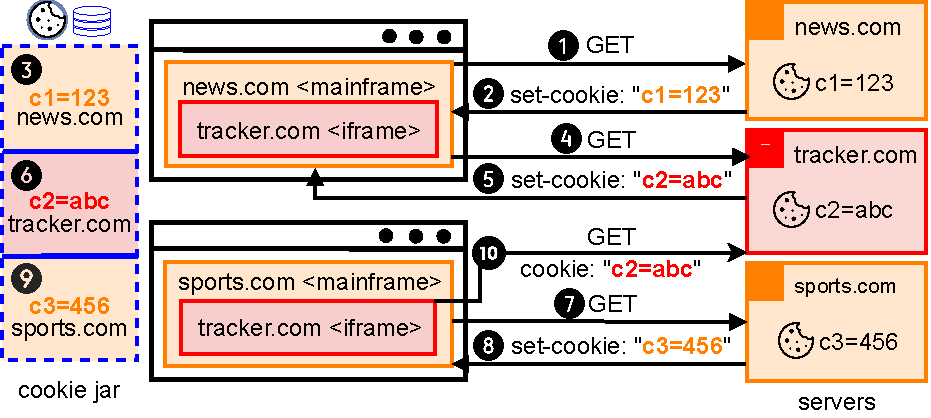
\includegraphics[width=1\linewidth]{figures/tracking-mechanisms-cookie.pdf}
    \caption{Cookie-based Tracking.}
    \label{subfig:cookie-tracking}
\end{figure}

%%
Cookie-based tracking relies on the browser's cookie jar \symStorage\ to maintain state, with cookies set and retrieved via HTTP headers \symSharing\ or JavaScript (JS) APIs such as \texttt{document.cookie} \symExecution.
%
For example, in \autoref{subfig:cookie-tracking}, \texttt{news.com} and \texttt{sports.com} both include iframes with ads from \texttt{tracker.com}.
%
As a result, the user’s browser will send the same \texttt{tracker.com} cookie with requests to load the iframes on both pages.
%
On \texttt{tracker.com} server's side, these two requests can be attributed to the same user and combined with additional information about the user-visited website.
% (from the HTTP Referrer header or query parameters passed along when the request to load the iframe is made).
%%
Cookies were adopted for cross-site tracking almost immediately after their introduction in the 1990s~\cite{montulliHTTPStateManagement1997}, prompting early privacy concerns~\cite{kristolHTTPCookiesStandards2001,SenatorRaisesPrivacy2001}.
%
Despite these concerns, third-party cookie-based tracking remained dominant for nearly two decades, becoming both widespread and concentrated among a few third parties~\cite{krishnamurthyPrivacyDiffusionWeb2009,lernerInternetJonesRaiders2016,englehardtOnlineTracking1millionsite2016,yuTrackingTrackers2016,karajWhoTracksMeShedding2019}.

%%
Browsers mediate cookie access based on the context in which they are set
---classifying them as first-party or third-party cookies---determining which resources and domains can access specific cookies
~\cite{beugin2024WebAlmanac2024,singhIncoherenciesWebBrowser2010,mdnSameoriginPolicySecurity2024}.
%
As Safari and Firefox began blocking or partitioning third-party cookies by default~\cite{TrackingPreventionWebKit2020,mdnThirdpartyCookiesPrivacy2024}  between 2018 and 2020 (\autoref{sec:stateful-defenses}), tracking shifted to the first-party context---nearly 90\% of websites now set first-party tracking cookies, 96\% of which are set by third-party scripts, making browsing with third-party cookies disabled largely indistinguishable from the pre-blocking web~\cite{munirCookieGraphUnderstandingDetecting2023,vekaria2024WebAlmanac2024,linBrowsingThirdPartyCookies2024}.
%
Meanwhile, trackers continue exploiting browser- and protocol-level edge cases such as opting out of \texttt{SameSite=Lax} and instead relying on \texttt{SameSite=None} cookies~\cite{khodayariStateSameSiteStudying2022}, to retain stateful tracking capabilities~\cite{bashirHowTrackingCompanies2018}.


%%
\subsubsection{Cookie Respawning}
\label{sec:stateful-techniques-cookie-respawning}
%%
Once a user clears their cookies, a tracker that has stashed the same identifier somewhere else in the browser can rewrite it back into the cookie jar, ``\textit{respawning}'' or reconstructing the identifier and creating a so-called ``supercookie'' or ``evercookie''~\cite{ayensonFlashCookiesPrivacy2011,soltaniFlashCookiesPrivacy2009,acarWebNeverForgets2014} as described in~\autoref{sec:stateful-defenses-evercookie}.
%
Respawning was first demonstrated at scale using Flash Local Shared Objects and other legacy plugin storage~\cite{acarWebNeverForgets2014,englehardtOnlineTracking1millionsite2016}, and later shown to also draw on browser fingerprints themselves---a 2022 study measured a lower bound on fingerprint-based respawning by detecting it on 1,150 of the top 30K sites~\cite{fouadMyCookiePhoenix2022}.
%
More recently, respawning has expanded beyond the browser, leveraging cross-context state shared with native applications to recover identifiers~\cite{wessels2025hytrack} (further discussed in~\refappendix{sec:mixed-techniques}).
% The technique's most recent evolution moves respawning outside the browser altogether: HyTrack shows that Android's Custom Tabs and WebView components, which are designed to let a native app and the system browser share cookies for a seamless login experience, let a tracker resurrect a supercookie-like identifier across app reinstalls, browser switches, and even device backups~\cite{wessels2025hytrack}---a persistence guarantee no purely in-browser respawning technique has ever achieved.


%%
\subsubsection{Cookie Syncing}
\label{sec:stateful-techniques-cookie-syncing}%%
To exchange information about users across domains included on a webpage \symInclusion, third-party companies rely on \textit{cookie syncing}~\cite{acarWebNeverForgets2014}---first described by Olejnik et al.~\cite{olejnikSellingPrivacyAuction2014}---which synchronizes user identifiers maintained in each party's cookie jar \symStorage, most commonly shared via URL parameters embedded in redirects \symSharing\ between them, requiring script execution \symExecution\ to initiate the sync.
% Following from the previous example, let’s suppose there are 
If amongst two trackers (\texttt{tracker1.com} and \texttt{tracker2.com}), only \texttt{tracker1.com} is present on \texttt{news.com} as shown in \autoref{subfig:cookie-syncing}, it can share its user identifier stored in a third-party cookie by initiating a request to \texttt{tracker2.com} and adding it in the URL parameter. 
%
This would allow \texttt{tracker2.com} to know the identifier the user has for \texttt{tracker1.com}, match it with the user identifier of \texttt{tracker2.com}, and communicate server-to-server to further merge the information collected about this user by \texttt{tracker1.com} and \texttt{tracker2.com}. 

%
Earlier works formalized cookie syncing detection~\cite{acarWebNeverForgets2014,englehardtOnlineTracking1millionsite2016,bashirTracingInformationFlows2016}, which has since been refined~\cite{papadopoulosCookieSynchronizationEverything2019} and scaled into automated, graph- and ML-based pipelines tracing identifier flows across the ecosystem~\cite{papadopoulosCookieSynchronizationEverything2019, iqbalKhaleesiBreakerAdvertising2022}.
%
Cookie syncing is not just confined to the third-party context~\cite{sanchez-rolaJourneyCenterCookie2021}, as identifiers in first-party cookies have been observed to be shared with hundreds of other third-party domains~\cite{munirCookieGraphUnderstandingDetecting2023,bahramiCOOKIEGUARDCharacterizingIsolating2024}.

\begin{figure}[htbp]
    \centering
    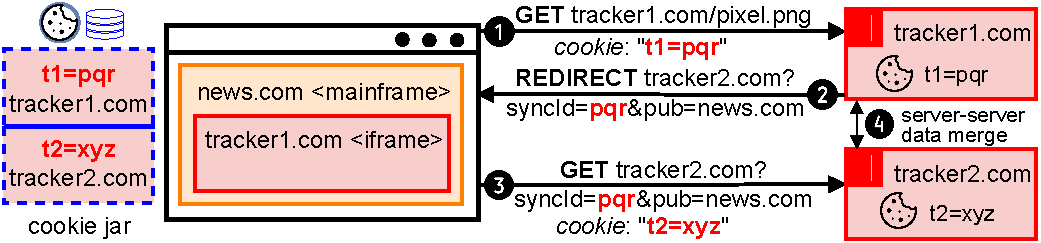
\includegraphics[width=1\linewidth]{figures/tracking-mechanisms-cookie-syncing.pdf}
    \caption{Cookie Syncing.}
    \label{subfig:cookie-syncing}
\end{figure}


%%
\subsubsection{Tracking Pixels/Tags}
\label{sec:stateful-techniques-tags}
%%
\textit{Tracking pixels}, traditionally referred to as 1x1 image elements embedded \symInclusion\ on a webpage, shared \symSharing\ user data with a tracking endpoint over HTTP traffic artifacts, enabling same- and cross-site tracking for analytics, ad (re)targeting, and conversion tracking
~\cite{Narayanan2017WebtapSpringer,englehardtOnlineTracking1millionsite2016}.
%
\autoref{subfig:tracking-scripts} represents a simple scenario where a tracking pixel from \texttt{tracker.com} is embedded on the homepage as well as on the \texttt{/signup} page of \texttt{news.com}, respectively collecting and sharing button clicks and form events with its own server, with the help of its tracking script.


\begin{figure}[htbp]
    \centering
    
\includegraphics[width=1\linewidth]{figures/tracking-mechanisms-tracking-tags.pdf}
    \caption{Tracking Scripts.}
    \label{subfig:tracking-scripts}
\end{figure}


Their prevalence and privacy risks have been measured extensively, from early archaeological studies of the tracking ecosystem~\cite{lernerInternetJonesRaiders2016,englehardtOnlineTracking1millionsite2016} to recent audits of their collection of personal data~\cite{huCharacterizingPixelTracking2019,bekosPIIxelLeaksPassive2025}.
%
As browser restrictions rendered third-party image-based pixels increasingly ineffective, modern tracking pixels have evolved into JS-based \textit{tracking tags} that execute \symExecution\ with the embedding site's first-party privileges to collect richer behavioral data~\cite{bekosHitchhikersGuideFacebook2023,munirCookieGraphUnderstandingDetecting2023}, while trackers increasingly obfuscate pixel behavior via falsified image dimensions, redirect chains, and encoded identifiers~\cite{huCharacterizingPixelTracking2019}.
%
Modern tags have also expanded in scope to support tag management, bot detection, session replays, and email tracking~\cite{senolLeakyFormsStudy2022,acarNoBoundariesData2020,englehardtNoBoundariesCredentials2018,englehardtNeverSignedThis2018,fouadMissedFilterLists2020}. Recent studies have shown deployments of the same vendor's tag to vary substantially across websites in their data collection~\cite{kiesermanTrackerInstallationsAre2025,bekosPIIxelLeaksPassive2025,ghaniPixelConfigLongitudinalMeasurement2026}.


%%
\begin{opbox}
Detecting the mere presence of a tracking tag is not enough to understand its capabilities---how do different configurations across sites and vendors determine what data is tracked, collected and shared, and how those settings evolve? 
What generalizable approaches can systematically measure tracking deployments across tags?
\end{opbox}

%%
\subsubsection{CNAME Tracking}
\label{sec:stateful-techniques-cname}
%%
Rather than embedding a third-party resource directly, a website can create a CNAME DNS record pointing a first-party subdomain (e.g., \textit{metrics.news.com}) to a third-party's infrastructure.
%
Because the browser only resolves \textit{metrics.news.com}, cookies set through this alias are treated as first-party \symStorage, allowing trackers to evade defenses that block third-party domains rather than DNS resolution~\cite{dimovaCNAMEGameLargescale2021} (a network protocol artifact). 
%
First documented in 2014~\cite{olejnikSellingPrivacyAuction2014,olejnikBidNotBid2014}, CNAME cloaking became widely adopted later in the decade as a response to browser anti-tracking measures. Deployed on roughly one in ten of the top-10k websites~\cite{dimovaCNAMEGameLargescale2021}, cloaked requests are indistinguishable from legitimate first-party traffic~\cite{dimovaCNAMEGameLargescale2021,chenCookieSwapParty2021}.

%%
% As browser-based defenses such as third-party cookie restrictions and community-based filterlist-powered content blocking have steadily eroded client-side tracking signals, the advertising industry has explicitly called for an architectural change. 
% %
% The IAB notes that client-side ad technology dependent on third-party code execution ``cannot be sustained as it stands today'' and advocates server-side architectures that ``eliminate client-side dependencies and mitigate ad-blocking threats''~\cite{iabtechlabTechLabTrusted2025}.
%
%%
More broadly, CNAME cloaking supports an emerging \emph{server-side tracking} paradigm, which reuses client-side pixel/tag instrumentation to collect tracking data but routes the resulting requests through a publisher-controlled first-party endpoint---often a CNAME-aliased or A/AAAA-record subdomain~\cite{jazlanSSTGuardDetectingCharacterizing2026}---before forwarding payloads to the tracker's backend via server-to-server communication, rendering client-side defenses ineffective~\cite{fouadDevilDetailsDetection2024}.
%
Major platforms including Google, Meta, and TikTok have already deployed conversion APIs adopting this architecture, and analysis suggests comparable tracking fidelity to client-side approaches
~\cite{fraihiClientsideServersideTracking2024}.

\begin{opbox}
As tracking logic shifts from client-side to server-side, it removes the vantage point that the research community has relied on to detect and mitigate online tracking. How can we characterize the prevalence and behavior of server-side tracking technologies, and what new methodologies (e.g., differential traffic probing, cooperation with first parties) are needed to study and defend against it?
\end{opbox}



%%
\subsubsection{Navigational Tracking via Link Decorations}
\label{sec:stateful-techniques-link-decorations}

%%
\textit{Link decorations} allow sharing identifiers \symSharing\ via query parameters, resource path segments, or URL fragments appended to an otherwise ordinary navigation as depicted in \autoref{subfig:navigational-tracking}.
%
The technique dates to the standardization of query parameters (RFC~1630, 1994) and the \texttt{Referer} header (RFC~1945, 1996), but became a deliberate tracking channel with the introduction of UTM parameters by Urchin/Google Analytics in 2005 and Google's click ID (\texttt{gclid}) in 2010.
%
As browsers began restricting third-party cookies, major ad platforms followed with their own click IDs (e.g., Meta's \texttt{fbclid}, Microsoft's \texttt{msclkid}), and over 70\% of websites now use decorations to share user data such as first-party cookies and email across navigations~\cite{munirPURLSafeEffective2024,koopInDepthEvaluationRedirect2020}.
%
Similarly, link \textit{shimming} involves a first-party rewriting the outbound links with decorations to route clicks through its own domain before redirecting.
%
While used for HTTPS upgrading or malicious-URL blocking, it equally enables the first party to log every outbound navigation~\cite{liShimShimmenyEvaluating2020}.
%
A recent audit of the \texttt{Referer} header further shows that inconsistent browser enforcement of Referrer-Policy still permits the cross-site identifier leakage the policy was designed to prevent~\cite{zagiReferrerPolicyImplementation2025}.

\begin{figure}[htbp]
    \centering
    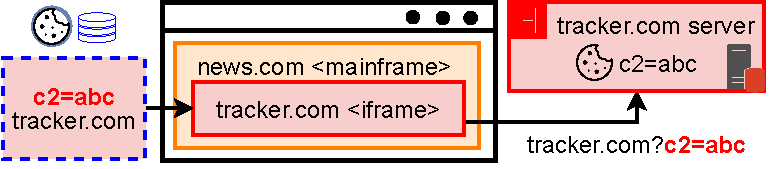
\includegraphics[width=1\linewidth]{figures/tracking-mechanisms-navigational-tracking.pdf}
    \caption{Navigational Tracking.}
    \label{subfig:navigational-tracking}
\end{figure}

%%
\subsubsection{Bounce Tracking}
\label{sec:stateful-techniques-bounce-tracking}

%%
\textit{Bounce tracking} is another navigation-based mechanism that renders third-party cookie blocking ineffective~\cite{kellyBounceTrackingMitigations2022}.
%
Unlike link shimming, where a first party rewrites outbound links to log clicks through its own domain~\cite{liShimShimmenyEvaluating2020}, bounce tracking specifically involves navigating a \emph{third-party} tracker's domain in first-party context, momentarily surfacing it during a redirect chain so it can read and write identifiers (via JS APIs \symExecution\ or cookie headers \symSharing) that persist in first-party storage \symStorage, linking them with website-specific identifiers for cross-site tracking.
%
Bounce chains can involve two (\texttt{news.com} $\rightarrow$ \texttt{tracker.com} $\rightarrow$ \texttt{news.com}) or more unrelated sites, propagating a stable user identifier across multiple unrelated websites.
%
\autoref{subfig:bounce-tracking} shows a typical \textbf{bounce-tracking} sequence:
%
\ding{182} a third-party script on \texttt{news.com} reads first-party identifier(s) stored under \texttt{news.com} and
%
\ding{183} includes them in the request to \texttt{tracker.com}.
%
\ding{184} Browser redirects to \texttt{tracker.com}, either by a user click, automatically (e.g., \texttt{window.location.href="...";}, or a \texttt{<meta http-equiv="refresh">}).
%
\ding{185} Once loaded as a \emph{first party}, \texttt{tracker.com} reads the identifier from the URL or merges it with an existing cookie, rewriting the URL to its final destination (e.g., back to \texttt{news.com} or other domain), embedding the consolidated identifier.
%
\ding{186} The browser navigates to \texttt{news.com}; the tracker’s script there extracts the identifier from the decorated URL and 
%
\ding{187} stores it in \texttt{news.com}’s first-party storage, completing the cross-context or cross-site linkage if redirected to same first-party or a different domain.
%
Due to usability disruptions and defensive measures, bounce tracking is not as widely pervasive as link decorations~\cite{iqbalKhaleesiBreakerAdvertising2022}, but both mechanisms are often used together.
%
Measurements in 2020 found that 11.6\% of sites use one of the top 100 redirectors~\cite{koopInDepthEvaluationRedirect2020}, and in 2022 such identifiers were present in 8.1\% of crawled navigations~\cite{randallMeasuringUIDSmuggling2022}.

\begin{figure}[htbp]
    \centering
    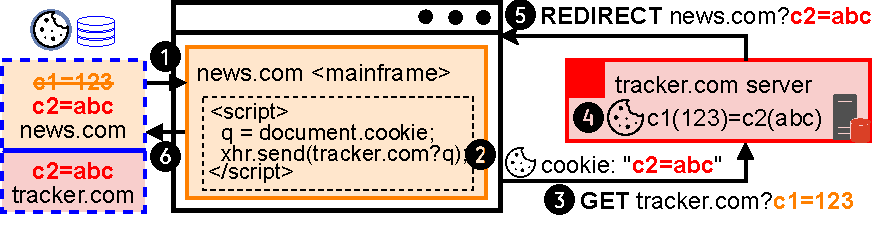
\includegraphics[width=1\linewidth]{figures/tracking-mechanisms-bounce-tracking.pdf}
    \caption{Bounce Tracking.}
    \label{subfig:bounce-tracking}
\end{figure}
\begin{comment}
% \begin{enumerate}[label=(\roman*)]
\begin{dingautolist}{182}
  \item A third-party script on \texttt{news.com} reads any first-party identifier already stored under \texttt{news.com}.
  \item Identifier is included in the request to \texttt{tracker.com}.
  \item Browser redirects—either by a user click or automatically (e.g., \texttt{window.location.href="...";} or a \texttt{<meta http-equiv="refresh">})—to \texttt{tracker.com}.
  \item Once loaded as a \emph{first party}, \texttt{tracker.com} reads the identifier from the URL or merges it with an existing cookie, rewriting the URL to its final destination (e.g., \texttt{sports.com}), embedding the consolidated identifier.
  \item Browser navigates on to \texttt{sports.com}; the tracker’s script there extracts identifier from the decorated URL and stores it in \texttt{sports.com}’s first-party storage, completing the cross-site linkage.
\end{dingautolist}
\end{comment}

\begin{opbox}
Each generation of navigational tracking, from UTM parameters to click IDs to bounce tracking, emerged as its predecessor was restricted. How will trackers adapt these channels to complement server-side tracking and how can we defend against it?
\end{opbox}


%%
\noindent Overall, every time an anti-tracking defense closes off one tracking vector, stateful trackers relocate tracking a layer further from the browser---from third-party cookies, to first-party cookies and synced identifiers, to DNS aliases, to server-side.

\begin{opbox}
As tracking logic keeps moving away from the browser, the community's tooling
% that majorly instruments the browser, 
needs to advance with it, or risk studying an increasingly small unrepresentative slice of how users are actually tracked.
\end{opbox}


%%
\para{Session Replays.}
Session replay (or recording) scripts capture detailed user interactions such as keystrokes, mouse, and scrolling movements, along with the full content of the visited pages.
%
This allows publishers to record and playback visits as if they are ``looking over [visitors’] shoulders’’, for purposes including marketing, analytics, and troubleshooting~\cite{AdvancedUsageInspectlet}.
%
However, these scripts can also capture sensitive personal data filled out by visitors~\cite{acarNoBoundariesData2020,senolLeakyFormsStudy2022,yuGotSickTracked2022}, while redaction measures offered by session replay vendors are often fragile and limited in effectiveness~\cite{englehardtNoBoundariesCredentials2018,acarNoBoundariesData2020}.










%%
\subsection{Stateless Tracking}
\label{sec:stateless-tracking}

%%
Unlike stateful tracking, \textit{stateless} tracking does not rely on stored identifiers but instead collects artifacts of the user's behavior, browser, or hardware to generate a fingerprint that correlates users across sites and sessions.
%
Nearly all stateless techniques are realized by exercising the \symExecution\ capability, with JavaScript running in the including context's privileges \symInclusion\ .
% ---hence their categorization also as ``JavaScript-based tracking'' (\autoref{sec:mixed-techniques-js-tracking}).

\begin{figure}[htbp]
    \centering
    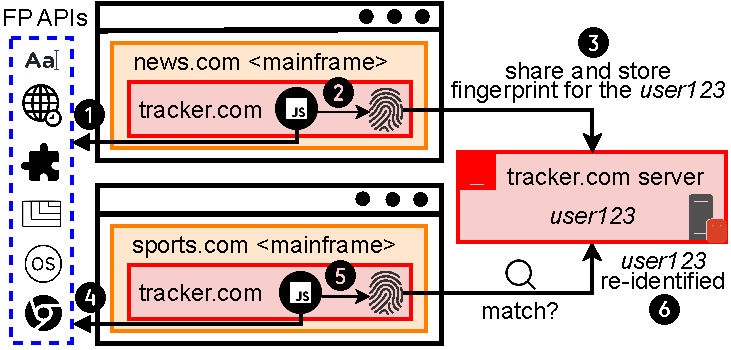
\includegraphics[width=0.85\linewidth]{figures/tracking-mechanisms-fingerprinting.pdf}
    \caption{Stateless Tracking via Fingerprinting.}
    \label{fig:stateless-tracking}
\end{figure}

%%
\para{Fingerprinting.} 
%
Fingerprinting corresponds to the gathering of information on users’ behavior (e.g., mouse movements, keystrokes), browser (e.g., version, screen size, installed fonts, GPU model, timezone and preferred languages), and hardware/OS in real-time via HTTP headers and JS APIs to identify users as depicted in~\autoref{fig:stateless-tracking}.
%
Several types of fingerprinting techniques exist based on the nature of the collected attributes.
%
Its use for tracking is hard to prevent due to the duality of fingerprinting (see~\refappendix{sec:need-for-fingerprinting}) which serves both constructive (e.g., bot and fraud detection) and destructive (e.g., tracking anonymous users) purposes. 
%
% This duality has hindered attempts to selectively block it (see~\refappendix{sec:need-for-fingerprinting}), with only recent work beginning to differentiate the intent, e.g., by using ad changes as a heuristic for fingerprinting-driven tracking~\cite{liuFirstEarlyEvidence2025}.
Recent work only began to differentiate intent, e.g., by using ad changes as a heuristic for fingerprinting-driven tracking~\cite{liuFirstEarlyEvidence2025}.

%%
\begin{opbox}
Can we automatically assign the purposes of trackers to determine fingerprinting intent and block only tracking use cases while allowing the benign ones?
\end{opbox}



%%
\subsubsection{Passive Fingerprinting} 
\label{sec:stateless-techniques-passive-fingperinting}
%
% Instead of actively probing the browser, 
\textit{Passive fingerprinting} exploits metadata attached to every request---most commonly IP address and User-Agent string (IPUA).
%
Despite its instability across networks, IP alone, or combined with minimal additional signals, can identify users~\cite{mishraDontCountMe2020,klineStructureCharacteristicsUser2017}, and even IPv6 address rotations intended to improve privacy is undermined by predictable ISP schedules and stable interface-identifier components~\cite{ryeFollowScentDefeating2021}.
%
Recent User-Agent reduction efforts have partially shrunk this surface, but remaining passive signals and Chrome's new Client Hints API still carry substantial identifying information~\cite{eckersleyHowUniqueYour2010,senolUnveilingImpactUserAgent2023,wieflingPrivacyMeasureTurned2024}.



%%
\subsubsection{Browser Fingerprinting} 
\label{sec:stateless-techniques-browser-fingperinting}

%%
\textit{Browser fingerprinting} actively probes browser APIs to collect configuration information about the browser, device, and OS.
%
Since the first academic work on browser fingerprinting in 2009~\cite{mayerAnyPersonPamphleteer2009} and the Electronic Frontier Foundation's Panopticlick shortly after~\cite{eckersleyHowUniqueYour2010}, researchers have extensively studied its impact on privacy and diversity~\cite{laperdrixBeautyBeastDiverting2016,gomez-boixHidingCrowdAnalysis2018}, its evolution and stability over time~\cite{vastelFPSTALKERTrackingBrowser2018}, its detection~\cite{suAutomaticDiscoveryEmerging2023,nomoto2023browser}, and discovered abusable browser APIs~\cite{olejnikLeakingBatteryPrivacy2016,dasWebsSixthSense2018,linFashionFauxPas2023,huygheFPRainbowFingerprintBasedBrowser2025}.
%
We refer readers to Laperdrix et al.'s SoK~\cite{laperdrix2020browser} for a comprehensive understanding of foundational aspects of browser fingerprinting.
%
% In 2013, fingerprinting was observed on $\sim$1\% of the top 10K websites~\cite{nikiforakisCookielessMonsterExploring2013} and $\sim$400 of the top 1M websites~\cite{acarFPDetectiveDustingWeb2013}. 
%
Over the years, its prevalence has grown steadily~\cite{nikiforakisCookielessMonsterExploring2013,acarFPDetectiveDustingWeb2013,englehardtOnlineTracking1millionsite2016,iqbalFingerprintingFingerprintersLearning2021}. 
%
% Prevalence has grown steadily, from $\sim$1\% of the top 10K sites in 2013~\cite{nikiforakisCookielessMonsterExploring2013,acarFPDetectiveDustingWeb2013} to 10\% of the top 100K (30\% of the top 1K) by 2021~\cite{iqbalFingerprintingFingerprintersLearning2021}, 
% with adoption concentrated among third parties and spanning diverse browser APIs~\cite{englehardtOnlineTracking1millionsite2016,dasWebsSixthSense2018}.
%
Browser fingerprints are inherently unstable, with 80\% of instances changing within 10 days~\cite{vastelFPSTALKERTrackingBrowser2018,liWhoTouchedMy2020}. 
%
So trackers often link evolving fingerprints by combining them with stateful techniques such as cookie respawning~\cite{fouadMyCookiePhoenix2022} (\autoref{sec:stateful-techniques-cookie-respawning}). %, as detected on 1,150 of the top 30K sites~\cite{fouadMyCookiePhoenix2022}.
%
Meanwhile, the exploitable surface continues to widen beyond Canvas, WebGL, and Audio APIs~\cite{chaliseYourSpeakerMy2022}: permission states~\cite{nomoto2023browser}, CSS and font-rendering differences~\cite{linFashionFauxPas2023}, divergent JS execution across platforms~\cite{zafarSameScriptDifferent2025}, and, even privacy-hardening switches themselves~\cite{huygheFPRainbowFingerprintBasedBrowser2025}.
%
Conclusions from prior studies about fingerprint uniqueness vary with dataset scale, 
% (from 470K~\cite{eckersleyHowUniqueYour2010} to 1.5B fingerprints~\cite{wuHimManyFaces2023}), 
and it remains unclear whether they generalize across devices, populations~\cite{berkeHowUniqueWhose2025,pradeepNotYourAverage2023}, or real browsing conditions~\cite{muthu2025beyond,deuserBrowsingUnicityLimits2020}, rendering its purpose and integration within live systems poorly understood.
%
% While existing research has shown how fingerprinting enables tracking and security, its real purposes and integration within live systems remain poorly understood.

%%
\begin{opbox}
What is the real impact of fingerprinting at scale, on vulnerable populations (e.g., minorities, children, marginalized), and paired with other techniques?
\end{opbox}


%%
\subsubsection{Hardware Fingerprinting} 
\label{sec:stateless-techniques-hardware-fingperinting}

%%
\textit{Hardware fingerprinting} exploits physical-layer variations to identify devices, first demonstrated via TCP clock-skew measurements~\cite{kohnoRemotePhysicalDevice2005} and later extended to the web through JS-accessible device~\cite{nikiforakisCookielessMonsterExploring2013} and cross-browser OS/hardware~\cite{caoCrossBrowserFingerprintingOS2017} properties.
%
Researchers have since demonstrated fingerprinting of specific components including CPUs~\cite{trampertBrowserBasedCPUFingerprinting2022,sanchez-rolaClockClockTimeBased2018}, GPUs via rendering variations~\cite{laorDRAWNAPARTDevice2022}, DRAM via Rowhammer-styled access patterns~\cite{venugopalanFPRowhammerDRAMBasedDevice2024}, and kernel-level PRNG state~\cite{kleinCrossLayerAttacks2021,kol2023device}.
%
The mobile ecosystem expands this surface through BLE frames \cite{martinHandoffAllYour2019} and motion, orientation, and acoustic sensors that are accessible without permission prompts~\cite{zhouAcousticFingerprintingRevisited2014,zhang2019sensorid,dasWebsSixthSense2018}.
% \cite{deyAccelPrintImperfectionsAccelerometers2014,zhang2019sensorid,zhouAcousticFingerprintingRevisited2014,dasWebsSixthSense2018}.
%
% On the passive end, Apple's Continuity devices constantly broadcast identifying BLE frames that correlate across MAC address rotations, enabling nearby tracking despite randomization~\cite{martinHandoffAllYour2019}.

%%
\begin{opbox}
Hardware fingerprinting exploits manufacturing variations that cannot be mitigated via software updates. What principled abstractions or hardware-software co-designs can provably bound the fingerprintable information leaking through device APIs, while preserving functionality and security properties (e.g., hardware attestation, PUFs) that rely on the same physical-layer uniqueness?
\end{opbox}


%%
\subsubsection{Behavioral Fingerprinting} 
\label{sec:stateless-techniques-behavioral-fingperinting}

%%
Fine-grained interaction signals such as mouse movements, keystroke patterns, and touch gestures can reliably distinguish users and support continuous authentication~\cite{attererKnowingUsersEvery2006,zhengEfficientUserVerification2011,leivaMyMouseMy2021,fereidooniAuthentiSenseScalableBehavioral2023}.
Mobile touch dynamics alone offers roughly 20 bits of entropy without requiring any permissions~\cite{masoodTouchYoureTrappcked2018}.
%
% These signals extend beyond input dynamics. 
%
Keystroke patterns link users across devices~\cite{yuanCrossdeviceTrackingIdentification2018}, engagement patterns correlate users across unrelated sites~\cite{gogaExploitingInnocuousActivity2013}, and form-filling behavior is collected at scale via session replay technologies~\cite{linFillBlanksEmpirical2020,cuiUnderstandingPrivacyNorms2025,acarNoBoundariesData2020}.
%
Recent work has begun assessing how well behavioral methods hold up as a general-purpose fingerprinting signal~\cite{crichtonRethinkingFingerprintingAssessment2025}.

%%
\begin{opbox}
As AI agents automate web browsing, they will impact behavioral fingerprinting techniques, raising questions on its effectiveness, attribution, and evasion.
\end{opbox}


%%
\subsubsection{Extension Fingerprinting} 
\label{sec:stateless-techniques-extension-fingperinting}

%%
Browser \textit{extension fingerprinting} infers the presence of specific extensions, which can reveal sensitive user attributes (e.g., health conditions, religion)~\cite{karamiCarnusExploringPrivacy2020}.
%
Early approaches relied on probing web-accessible resources (WARs) that extensions expose~\cite{starovXHOUNDQuantifyingFingerprintability2017,starovExtendedTrackingPowers2017,starovUnnecessarilyIdentifiableQuantifying2019}, but because static WAR probing is comparatively easy to randomize away~\cite{trickelEveryoneDifferentClientside2019}, research shifted towards \textit{behavioral} extension fingerprinting---inferring extensions through side-effects during execution such as information leakage across components~\cite{chenMystiqueUncoveringInformation2018}, user-triggered actions~\cite{solomosDangersHumanTouch2022}, injected CSS~\cite{laperdrixFingerprintingStyleDetecting2021}, and transient DOM edits~\cite{solomosEscapingConfinesTime2022}.
%
Behavioral fingerprints have proven far more resilient, with 88\% remaining effective even against dedicated countermeasures \cite{karamiCarnusExploringPrivacy2020}, making defense fundamentally harder than blocking resource enumeration.
%
Most recently, even ad blockers have been shown to be fingerprintable through scriptless, filter-list-driven side effects, where customizing a rule set paradoxically shrinks a user's anonymity set~\cite{chehade2025double}.

%%
\begin{opbox}
How can future browser architectures and extension frameworks be co-designed so that extensions can modify page behavior without exposing detectable side-effects, and what privacy guarantees can such designs formally provide against an adaptive adversary that combines behavioral, stylistic, and scriptless fingerprinting vectors?
\end{opbox}


%%
\subsubsection{Side-channel Fingerprinting} 
\label{sec:stateless-techniques-side-channel-fingperinting}

%%
\textit{Side-channel fingerprinting} exploits unintended information leakage across browser, network, and hardware layers to track users without relying on stored identifiers or active probing.
%
Together, this line of work has suggested a trajectory away from brittle single-mechanism attacks and toward compositional and cross-layer side channels that that exploit performance optimizations, shared infrastructure, and user interactions.
%
Generally, side-channel attacks are challenging to detect and could be equally difficult to mitigate.


%%
\para{Kernel-based Side-channels.}
%
At the OS level, process-accounting interfaces leak enough about recent activity to fingerprint browsing history from kernel artifacts alone~\cite{janaMementoLearningSecrets2012}. 
%
Additionally, Linux's shared kernel PRNG state lets attackers correlate DNS and TCP/IP behavior into a stable device identifier that persists until reboot~\cite{kleinCrossLayerAttacks2021,kol2023device}.


%%
\para{Network-based Side-channels.}
%
Encrypted traffic still leaks sensitive state through observation \symObservation\ of network-level artifacts such as packet sizes and timing~\cite{chenSideChannelLeaksWeb2010,gonzalezUserProfilingTime2016}, TLS client certificates act as persistent supercookies rarely revoked by users~\cite{foppeExploitingTLSClient2018}, and QUIC's connection-migration feature lets server-chosen connection IDs be encoded and visible to on-path observers even as clients change networks~\cite{syQUICLookWeb2019}. 


%%
\para{Storage-based Side-channels.}
%
Multiple browser caching layers such as favicon cache~\cite{solomosTalesFaviconsCaches2021}, HTTP cache, ETags, Alt-Svc~\cite{mishraDejaVuAbusing2021}, and DNS resolver cache~\cite{klein2019dns} were independently proven abusable as cross-context identifier stores \symStorage, since none were originally designed with cross-site isolation in mind.
%
More recent works have demonstrated that shared browser resource pools create cross-context timing channels in all major browsers~\cite{snyderPoolPartyExploitingBrowser2023} and automated feature-testing frameworks have surfaced previously unknown tracking vectors by probing browser features systematically~\cite{aliNavigatingMurkyWaters2023}.


%%
\para{Timing-based Side-channels.}
%
Timing attacks on the web date to Felten and Schneider's 2000 demonstration that cache behavior reveals browsing history~\cite{feltenTimingAttacksWeb2000}, and have since escalated through JS-driven CPU cache attacks~\cite{orenSpySandboxPractical2015}, browser-level side-channels independent of network conditions~\cite{van2015clock}, and concurrency-based timing that eliminates the need for absolute clocks~\cite{van2020timeless}.
%
Most notably, Chrome's Site Isolation---introduced specifically to counter Spectre---was itself shown to introduce new cross-origin timing side-channels~\cite{jinTimingBasedBrowsingPrivacy2022}.


%%
\begin{opbox}
Major browser features added for performance or security have often retrospectively introduced a tracking side-channel. Can browsers move from reactive patching to proactive side-channel auditing of new APIs and architectural changes before deployment? How can researchers build automated discovery frameworks directly integrable into the browser feature review process?
\end{opbox}


\begin{figure*}[!ht]
    \centering
    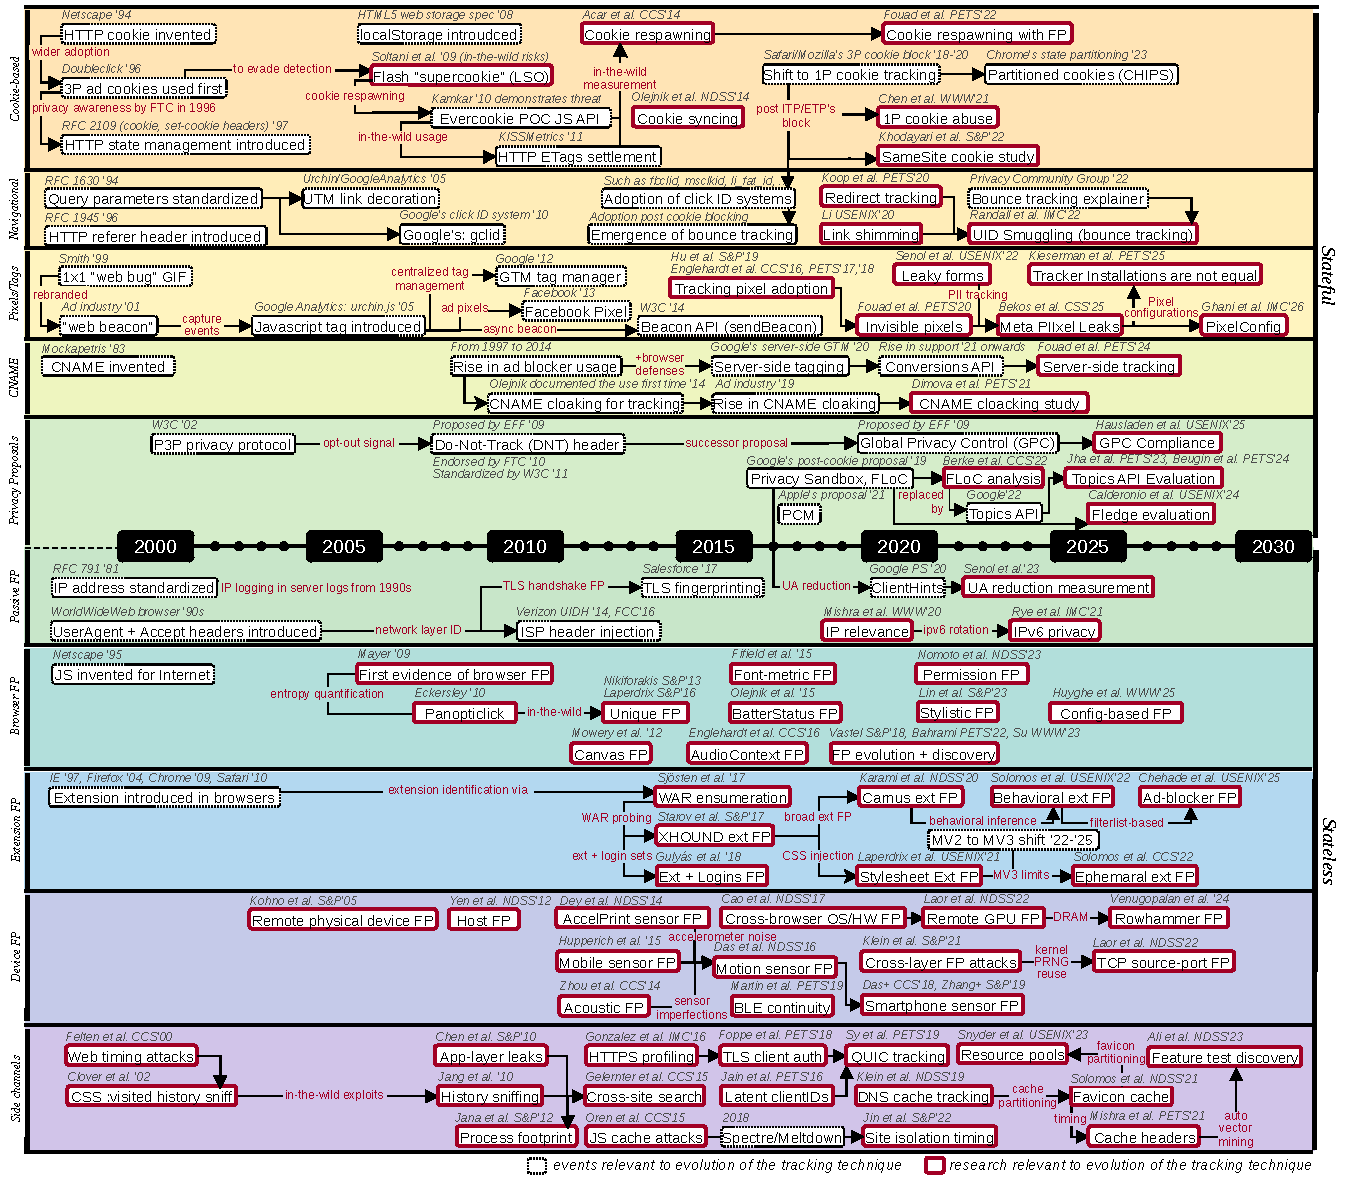
\includegraphics[width=1\linewidth]{long-version/evolution-tracking-techniques.pdf}
    \caption{Evolution of research on stateful and stateless web tracking techniques.}
    \label{fig:evolution-techniques}
\end{figure*}



\subsection{Mixed Tracking Techniques}
\label{sec:mixed-techniques}

%%
Prior stateful and stateless approaches can also be combined to track users across contexts---bridging identity across login boundaries, devices, browsers, and native apps. We refer to these techniques as mixed tracking.

\subsubsection{JavaScript-based Tracking}
\label{sec:mixed-techniques-js-tracking}

%%
% JavaScript is the unifying substrate of both stateful and stateless web tracking. 
%
JavaScript can be used to read and write browser cookies and storage for persistence by stateful techniques while also be used to probe browser APIs to construct a fingerprint by stateless techniques.
%
Although JS-based approaches don't constitute a different tracking technique, it is included here as a canonical example of mixed tracking in practice.


%%
\subsubsection{Authentication-based Tracking}
\label{sec:mixed-techniques-auth-tracking}

%%
Authentication creates a deterministic, cross-context identifier (an account or email address) far more durable than any cookie or fingerprint.
%
Logged-in users are served more third-party trackers and personalized content~\cite{kaizerCharacterizingWebsiteBehaviors2016}, and logged-in pages exhibit more fingerprinting than other pages on the same site, suggesting trackers use authentication to link a stateless fingerprint to stable account identifiers to extend identification into anonymous sessions~\cite{senolDoubleEdgedSword2024}.
%
Moreover, OAuth-based single sign-on itself routinely leaks identifying information to identity providers and relying parties~\cite{dimovaEverybodysLookingSSOmething2023}.
%
As email addresses survive cookie clears and device changes, first parties increasingly hash and share them with advertising partners to build cross-site identity graphs that restore the linkage that third-party cookie restrictions were designed to prevent.


%%
\subsubsection{Cross-device Tracking}
\label{sec:mixed-techniques-cross-device}

%%
When deterministic identifiers are unavailable (e.g., logged out state), trackers fall back to probabilistic signals to link activity across devices---shared IP addresses, browsing patterns~\cite{caoCrossBrowserFingerprintingOS2017}, and behavioral features such as typing dynamics~\cite{yuanCrossdeviceTrackingIdentification2018}.
%
These signals are combined into proprietary \textit{cross-device graphs}, a practice found to be largely opaque to both users and regulators~\cite{zimmeckPrivacyAnalysisCrossdevice2017,brookmanCrossDeviceTrackingMeasurement2017}.
%
Because probabilistic identifiers are inherently noisy (e.g., ISPs dynamically rotate and share public IP addresses across households), trackers apply heuristics such as ignoring commercial, private, and proxied IP ranges or setting temporal thresholds to filter false matches.

%%
\begin{opbox}
Given the lack of ground truth and diversity of proprietary linking algorithms forming cross-device identity graphs, how can cross-device tracking be reliably measured and systematically attributed to uncover specific signals used by different trackers?
\end{opbox}



%%
\subsubsection{Other Cross-Context Tracking}
\label{sec:mixed-techniques-cross-context}

%%
Trackers also bridge contexts within the same device.
%
Cross-browser fingerprinting uses OS- and hardware-level features stable across browsers to link users across browser boundaries~\cite{caoCrossBrowserFingerprintingOS2017}.
%
On mobile, Android Custom Tabs and WebViews share the browser's cookie jar with native apps, letting a tracker plants an identifier in one context that resurfaces in the other, surviving app reinstalls and device backups~\cite{wessels2025hytrack}.
%
% A complementary vector operates without any shared cookie jar, 
Recently, some native apps and in-browser scripts have been found to silently link identities by communicating over \texttt{localhost}, a channel neither the browser's permission model nor the OS sandbox was designed to police~\cite{localmess-usenix-sec-26}.
%
These vectors share a common root cause---OS- and browser-level integration points enabling legitimate app-to-web handoffs that are invisible to in-browser tracking defenses.

%%
\begin{opbox}
Cross-context tracking exploits integration boundaries between browsers, between apps and the web, and between user profiles that no single platform controls end to end. What architectural principles can unify isolation across these boundaries without fragmenting the seamless cross-context experiences users and developers expect?
\end{opbox}



